% Created by tikzDevice version 0.12.3.1 on 2023-02-19 11:34:00
% !TEX encoding = UTF-8 Unicode
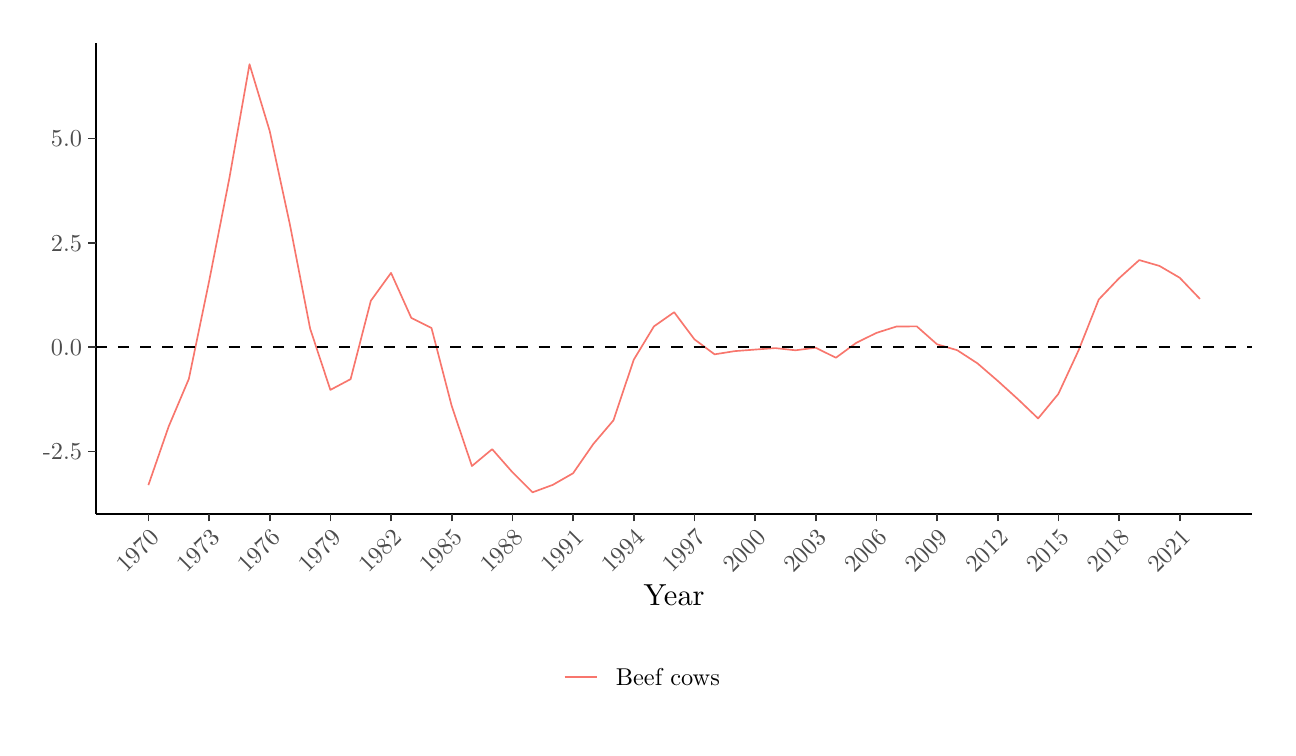
\begin{tikzpicture}[x=1pt,y=1pt]
\definecolor{fillColor}{RGB}{255,255,255}
\path[use as bounding box,fill=fillColor,fill opacity=0.00] (0,0) rectangle (448.07,252.94);
\begin{scope}
\path[clip] (  0.00,  0.00) rectangle (448.07,252.94);
\definecolor{drawColor}{RGB}{255,255,255}
\definecolor{fillColor}{RGB}{255,255,255}

\path[draw=drawColor,line width= 0.6pt,line join=round,line cap=round,fill=fillColor] (  0.00,  0.00) rectangle (448.07,252.94);
\end{scope}
\begin{scope}
\path[clip] ( 24.62, 77.31) rectangle (442.57,247.44);
\definecolor{fillColor}{RGB}{255,255,255}

\path[fill=fillColor] ( 24.62, 77.31) rectangle (442.57,247.44);
\definecolor{drawColor}{RGB}{248,118,109}

\path[draw=drawColor,line width= 0.6pt,line join=round] ( 43.62, 87.65) --
	( 50.93,108.77) --
	( 58.24,126.02) --
	( 65.54,161.22) --
	( 72.85,198.36) --
	( 80.16,239.71) --
	( 87.46,215.59) --
	( 94.77,181.73) --
	(102.08,144.13) --
	(109.38,122.05) --
	(116.69,125.93) --
	(124.00,154.25) --
	(131.30,164.33) --
	(138.61,148.08) --
	(145.92,144.40) --
	(153.22,116.25) --
	(160.53, 94.53) --
	(167.84,100.63) --
	(175.14, 92.32) --
	(182.45, 85.04) --
	(189.76, 87.74) --
	(197.07, 91.92) --
	(204.37,102.46) --
	(211.68,111.06) --
	(218.99,132.93) --
	(226.29,144.99) --
	(233.60,150.12) --
	(240.91,140.34) --
	(248.21,134.90) --
	(255.52,136.06) --
	(262.83,136.62) --
	(270.13,137.15) --
	(277.44,136.36) --
	(284.75,137.29) --
	(292.05,133.67) --
	(299.36,139.02) --
	(306.67,142.64) --
	(313.97,144.96) --
	(321.28,145.00) --
	(328.59,138.53) --
	(335.89,136.39) --
	(343.20,131.64) --
	(350.51,125.33) --
	(357.81,118.71) --
	(365.12,111.73) --
	(372.43,120.59) --
	(379.74,136.34) --
	(387.04,154.72) --
	(394.35,162.37) --
	(401.66,168.96) --
	(408.96,166.85) --
	(416.27,162.58) --
	(423.58,154.94);
\definecolor{drawColor}{RGB}{0,0,0}

\path[draw=drawColor,line width= 0.6pt,dash pattern=on 4pt off 4pt ,line join=round] ( 24.62,137.47) -- (442.57,137.47);
\end{scope}
\begin{scope}
\path[clip] (  0.00,  0.00) rectangle (448.07,252.94);
\definecolor{drawColor}{RGB}{0,0,0}

\path[draw=drawColor,line width= 0.6pt,line join=round] ( 24.62, 77.31) --
	( 24.62,247.44);
\end{scope}
\begin{scope}
\path[clip] (  0.00,  0.00) rectangle (448.07,252.94);
\definecolor{drawColor}{gray}{0.30}

\node[text=drawColor,anchor=base east,inner sep=0pt, outer sep=0pt, scale=  0.88] at ( 19.67, 96.74) {-2.5};

\node[text=drawColor,anchor=base east,inner sep=0pt, outer sep=0pt, scale=  0.88] at ( 19.67,134.44) {0.0};

\node[text=drawColor,anchor=base east,inner sep=0pt, outer sep=0pt, scale=  0.88] at ( 19.67,172.14) {2.5};

\node[text=drawColor,anchor=base east,inner sep=0pt, outer sep=0pt, scale=  0.88] at ( 19.67,209.85) {5.0};
\end{scope}
\begin{scope}
\path[clip] (  0.00,  0.00) rectangle (448.07,252.94);
\definecolor{drawColor}{gray}{0.20}

\path[draw=drawColor,line width= 0.6pt,line join=round] ( 21.87, 99.77) --
	( 24.62, 99.77);

\path[draw=drawColor,line width= 0.6pt,line join=round] ( 21.87,137.47) --
	( 24.62,137.47);

\path[draw=drawColor,line width= 0.6pt,line join=round] ( 21.87,175.17) --
	( 24.62,175.17);

\path[draw=drawColor,line width= 0.6pt,line join=round] ( 21.87,212.88) --
	( 24.62,212.88);
\end{scope}
\begin{scope}
\path[clip] (  0.00,  0.00) rectangle (448.07,252.94);
\definecolor{drawColor}{RGB}{0,0,0}

\path[draw=drawColor,line width= 0.6pt,line join=round] ( 24.62, 77.31) --
	(442.57, 77.31);
\end{scope}
\begin{scope}
\path[clip] (  0.00,  0.00) rectangle (448.07,252.94);
\definecolor{drawColor}{gray}{0.20}

\path[draw=drawColor,line width= 0.6pt,line join=round] ( 43.62, 74.56) --
	( 43.62, 77.31);

\path[draw=drawColor,line width= 0.6pt,line join=round] ( 65.54, 74.56) --
	( 65.54, 77.31);

\path[draw=drawColor,line width= 0.6pt,line join=round] ( 87.46, 74.56) --
	( 87.46, 77.31);

\path[draw=drawColor,line width= 0.6pt,line join=round] (109.38, 74.56) --
	(109.38, 77.31);

\path[draw=drawColor,line width= 0.6pt,line join=round] (131.30, 74.56) --
	(131.30, 77.31);

\path[draw=drawColor,line width= 0.6pt,line join=round] (153.22, 74.56) --
	(153.22, 77.31);

\path[draw=drawColor,line width= 0.6pt,line join=round] (175.14, 74.56) --
	(175.14, 77.31);

\path[draw=drawColor,line width= 0.6pt,line join=round] (197.07, 74.56) --
	(197.07, 77.31);

\path[draw=drawColor,line width= 0.6pt,line join=round] (218.99, 74.56) --
	(218.99, 77.31);

\path[draw=drawColor,line width= 0.6pt,line join=round] (240.91, 74.56) --
	(240.91, 77.31);

\path[draw=drawColor,line width= 0.6pt,line join=round] (262.83, 74.56) --
	(262.83, 77.31);

\path[draw=drawColor,line width= 0.6pt,line join=round] (284.75, 74.56) --
	(284.75, 77.31);

\path[draw=drawColor,line width= 0.6pt,line join=round] (306.67, 74.56) --
	(306.67, 77.31);

\path[draw=drawColor,line width= 0.6pt,line join=round] (328.59, 74.56) --
	(328.59, 77.31);

\path[draw=drawColor,line width= 0.6pt,line join=round] (350.51, 74.56) --
	(350.51, 77.31);

\path[draw=drawColor,line width= 0.6pt,line join=round] (372.43, 74.56) --
	(372.43, 77.31);

\path[draw=drawColor,line width= 0.6pt,line join=round] (394.35, 74.56) --
	(394.35, 77.31);

\path[draw=drawColor,line width= 0.6pt,line join=round] (416.27, 74.56) --
	(416.27, 77.31);
\end{scope}
\begin{scope}
\path[clip] (  0.00,  0.00) rectangle (448.07,252.94);
\definecolor{drawColor}{gray}{0.30}

\node[text=drawColor,rotate= 45.00,anchor=base east,inner sep=0pt, outer sep=0pt, scale=  0.88] at ( 47.91, 68.07) {1970};

\node[text=drawColor,rotate= 45.00,anchor=base east,inner sep=0pt, outer sep=0pt, scale=  0.88] at ( 69.83, 68.07) {1973};

\node[text=drawColor,rotate= 45.00,anchor=base east,inner sep=0pt, outer sep=0pt, scale=  0.88] at ( 91.75, 68.07) {1976};

\node[text=drawColor,rotate= 45.00,anchor=base east,inner sep=0pt, outer sep=0pt, scale=  0.88] at (113.67, 68.07) {1979};

\node[text=drawColor,rotate= 45.00,anchor=base east,inner sep=0pt, outer sep=0pt, scale=  0.88] at (135.59, 68.07) {1982};

\node[text=drawColor,rotate= 45.00,anchor=base east,inner sep=0pt, outer sep=0pt, scale=  0.88] at (157.51, 68.07) {1985};

\node[text=drawColor,rotate= 45.00,anchor=base east,inner sep=0pt, outer sep=0pt, scale=  0.88] at (179.43, 68.07) {1988};

\node[text=drawColor,rotate= 45.00,anchor=base east,inner sep=0pt, outer sep=0pt, scale=  0.88] at (201.35, 68.07) {1991};

\node[text=drawColor,rotate= 45.00,anchor=base east,inner sep=0pt, outer sep=0pt, scale=  0.88] at (223.27, 68.07) {1994};

\node[text=drawColor,rotate= 45.00,anchor=base east,inner sep=0pt, outer sep=0pt, scale=  0.88] at (245.19, 68.07) {1997};

\node[text=drawColor,rotate= 45.00,anchor=base east,inner sep=0pt, outer sep=0pt, scale=  0.88] at (267.11, 68.07) {2000};

\node[text=drawColor,rotate= 45.00,anchor=base east,inner sep=0pt, outer sep=0pt, scale=  0.88] at (289.03, 68.07) {2003};

\node[text=drawColor,rotate= 45.00,anchor=base east,inner sep=0pt, outer sep=0pt, scale=  0.88] at (310.95, 68.07) {2006};

\node[text=drawColor,rotate= 45.00,anchor=base east,inner sep=0pt, outer sep=0pt, scale=  0.88] at (332.87, 68.07) {2009};

\node[text=drawColor,rotate= 45.00,anchor=base east,inner sep=0pt, outer sep=0pt, scale=  0.88] at (354.79, 68.07) {2012};

\node[text=drawColor,rotate= 45.00,anchor=base east,inner sep=0pt, outer sep=0pt, scale=  0.88] at (376.71, 68.07) {2015};

\node[text=drawColor,rotate= 45.00,anchor=base east,inner sep=0pt, outer sep=0pt, scale=  0.88] at (398.63, 68.07) {2018};

\node[text=drawColor,rotate= 45.00,anchor=base east,inner sep=0pt, outer sep=0pt, scale=  0.88] at (420.56, 68.07) {2021};
\end{scope}
\begin{scope}
\path[clip] (  0.00,  0.00) rectangle (448.07,252.94);
\definecolor{drawColor}{RGB}{0,0,0}

\node[text=drawColor,anchor=base,inner sep=0pt, outer sep=0pt, scale=  1.10] at (233.60, 44.09) {Year};
\end{scope}
\begin{scope}
\path[clip] (  0.00,  0.00) rectangle (448.07,252.94);
\definecolor{fillColor}{RGB}{255,255,255}

\path[fill=fillColor] (181.59,  5.50) rectangle (285.61, 30.95);
\end{scope}
\begin{scope}
\path[clip] (  0.00,  0.00) rectangle (448.07,252.94);
\definecolor{drawColor}{RGB}{248,118,109}

\path[draw=drawColor,line width= 0.6pt,line join=round] (194.04, 18.23) -- (205.60, 18.23);
\end{scope}
\begin{scope}
\path[clip] (  0.00,  0.00) rectangle (448.07,252.94);
\definecolor{drawColor}{RGB}{0,0,0}

\node[text=drawColor,anchor=base west,inner sep=0pt, outer sep=0pt, scale=  0.88] at (212.55, 15.20) {Beef cows};
\end{scope}
\end{tikzpicture}
